\documentclass[11pt]{article}
\usepackage[margin=1.05in]{geometry}
\usepackage{amsmath,amssymb}
\usepackage{booktabs}
\usepackage{graphicx}
\usepackage[colorlinks=true,linkcolor=blue,citecolor=blue,urlcolor=blue]{hyperref}

\newcommand{\voles}{\texttt{voles}}
\newcommand{\flag}{\texttt{reuse\_adaptive\_blocks}}
\newcommand{\dd}{\,\mathrm{d}}

\title{The \flag{} flag:\\
trading bitwise reproducibility for assembly speed\\ on weakly singular kernels}
\author{Notes accompanying branch \texttt{adaptive-block-reuse}
(commit \texttt{946e709})}
\date{August 2026}

\begin{document}
\maketitle

\begin{abstract}
\noindent
The uniform-mesh weight-tensor assembly of the \voles{} callable-input
solvers (branch \texttt{fast-uniform-mesh}) reuses only blocks evaluated
by deterministic fixed-order quadrature, and re-evaluates every
adaptive-quadrature block per mesh row so that results match the
original code to rounding level. That policy leaves an $O(M)$
adaptive-quadrature cost that dominates weakly singular (Abel-kernel)
builds. This note documents an opt-in flag,
\flag{} (default \texttt{False}), that reuses the adaptive blocks too:
the Abel build cost drops by a further $\sim$40--140$\times$, at the
price of deviations from the default path of order $10^{-10}$ relative
--- larger than rounding, but \emph{no larger than the default path's
own internal inconsistency}, and six-plus orders of magnitude below
discretization error. We explain precisely where the deviations come
from (QUADPACK's tolerance-limited, branch-dependent adaptivity), report
measurements across every test-suite problem spec, and give the argument
for why the trade can be acceptable --- together with the cases where it
is not, which is why it is off by default.
\end{abstract}

\section{Interface and headline numbers}

All three callable-input solvers gain a keyword argument, default off:
\begin{center}
\texttt{function\_solve\_VIE\_1 / \_VIE\_2 / \_VIDE(\dots,
reuse\_adaptive\_blocks=False)}
\end{center}
Guarantees, enforced by tests: the flag is a strict no-op (bit-identical
output) on non-uniform meshes, for callable singularity locators, and
for smooth kernels (which have no adaptive blocks). It acts only on the
uniform-mesh convolution fast path, and only on weakly singular builds.

Headline measurements (Abel kernel $K=1/\sqrt{\pi u}$, VIE-1, $p=3$,
$T=20$; Apple-silicon laptop):
\begin{center}
\begin{tabular}{lccccc}
\toprule
$M$ & 80 & 320 & 1280 & 2560 & 5120\\
\midrule
default    & 0.53\,s & 2.06\,s & 8.35\,s & --- & ---\\
\flag{}    & 0.012\,s & 0.023\,s & 0.19\,s & 0.58\,s & 2.05\,s\\
\bottomrule
\end{tabular}
\end{center}
Both paths scale linearly in $M$; the flag removes the constant
($\approx$\,3\,p adaptive quadratures per row). Deviations between the
two paths, across every weakly singular problem spec of the test suite:
worst $2.2\times10^{-10}$ relative to solution scale
(Table~\ref{tab:battery}).

\section{Background: which blocks are adaptive, and why they were
re-evaluated per row}

On a uniform mesh with a convolution kernel, every weight-tensor block
\[
W[n,i,l,k]=\int_{t_l}^{t_{l+1}}K(\tau_{n,i}-s)\,
L_k\!\Bigl(\tfrac{s-t_l}{h}\Bigr)\dd s
\]
depends on $(n,l)$ only through the lag $n-l$, so one integrated row
determines the tensor (see the branch notes,
\texttt{fast\_uniform\_mesh\_notes.pdf}). Blocks are evaluated two ways:
smooth blocks by fixed-order Gauss--Legendre with a two-order acceptance
check --- a \emph{deterministic} rule whose equal-lag values agree to
$\sim10^{-15}$ --- and blocks touching a declared singularity (for an
Abel kernel: every diagonal block, whose upper integration limit is the
collocation point where $u=0$) by \texttt{scipy.integrate.quad}
(QUADPACK), plus occasional near-singular fallbacks. Under the
project's reproducibility policy (``optimizations must match the
original code to rounding level'') only the deterministic blocks are
reused; the adaptive ones are re-run per row with byte-identical calls.
Those per-row runs are exactly the residual cost the flag removes.

\section{What the flag changes}

With \flag{}\texttt{=True}:
\begin{enumerate}
\item the adaptive blocks of the single integrated row are computed at
  \emph{tightened} tolerance
  (\texttt{epsabs}=\texttt{epsrel}=$10^{-12}$, subdivision limit 200,
  instead of the library default $1.49\times10^{-8}$, limit 100);
\item the band-diagonal copy then stands for \emph{all} blocks --- the
  per-row repair loop is skipped entirely. The stored tensor is exactly
  Toeplitz, as the underlying mathematics says it should be.
\end{enumerate}
Nothing else changes: same classification, same GL machinery, same
downstream solve.

\section{Why the deviations exceed rounding level}

QUADPACK's adaptive algorithm guarantees its result only to the
requested tolerance, and the value it returns is a \emph{branchy}
function of its inputs: every subdivision and extrapolation decision
compares a floating-point error estimate against a threshold. Equal-lag
blocks in different rows are the same integral in exact arithmetic, but
the algorithm sees them at different absolute coordinates (endpoints and
$\tau-s$ arguments differing in their last bits); occasionally an
estimate lands on the other side of a branch, the subdivision tree
differs, and the result moves by up to the tolerance.

The decisive measurement: in the \emph{default} path, the $M$
mathematically identical diagonal blocks of an Abel build ($M=60$,
$T=20$, $p=3$) come back with a spread of
\[
\max_{i,k}\Bigl(\max_n W[n,i,n,k]-\min_n W[n,i,n,k]\Bigr)
= 3.4\times10^{-10},
\]
while the GL-clean lag-1 blocks agree to $9\times10^{-15}$. The default
path is itself inconsistent at the $10^{-10}$ level about quantities
that are exactly equal --- that inconsistency \emph{is} QUADPACK's
error, distributed across rows. Turning the flag on replaces the $M$
scattered values by one value per block; the on-vs-off difference is
therefore bounded by (and in practice sits at) the same
$10^{-10}$ scale. One caveat: the vector solvers use
\texttt{quad\_vec}, whose adaptive rule lacks QUADPACK's extrapolation
and carries larger genuine error on singular blocks; there the on/off
gap can reach $\sim10^{-7}$ at the weight level.

\section{The case that this can be acceptable}

\begin{figure}[t]
\centering
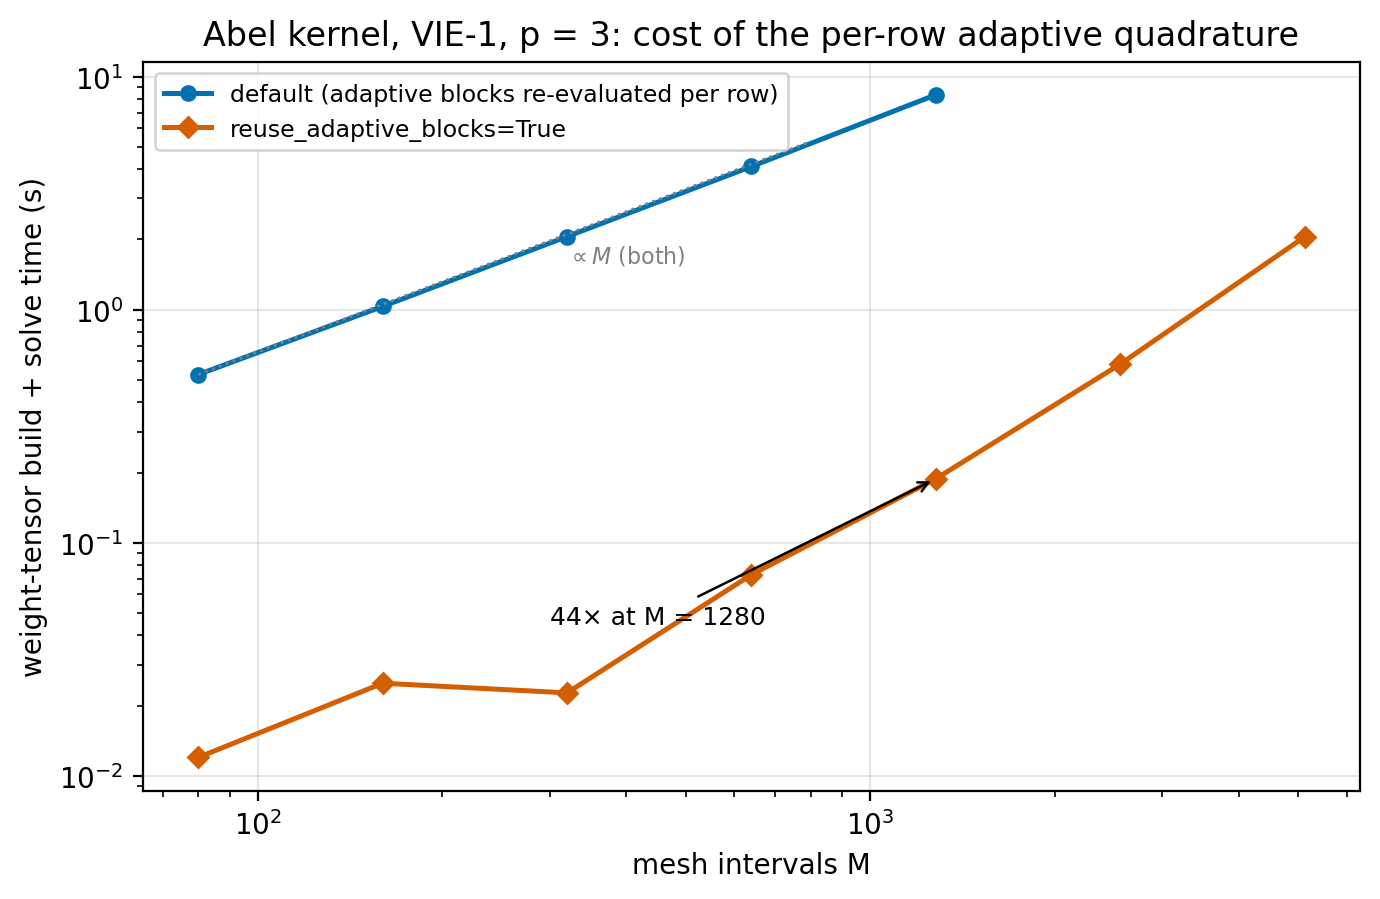
\includegraphics[width=0.78\textwidth]{plot_reuse_speedup.png}
\caption{Build cost with the flag off and on (Abel VIE-1, $p=3$). Both
paths are $O(M)$; the flag removes the per-row adaptive-quadrature
constant.}
\label{fig:speed}
\end{figure}

\begin{figure}[t]
\centering
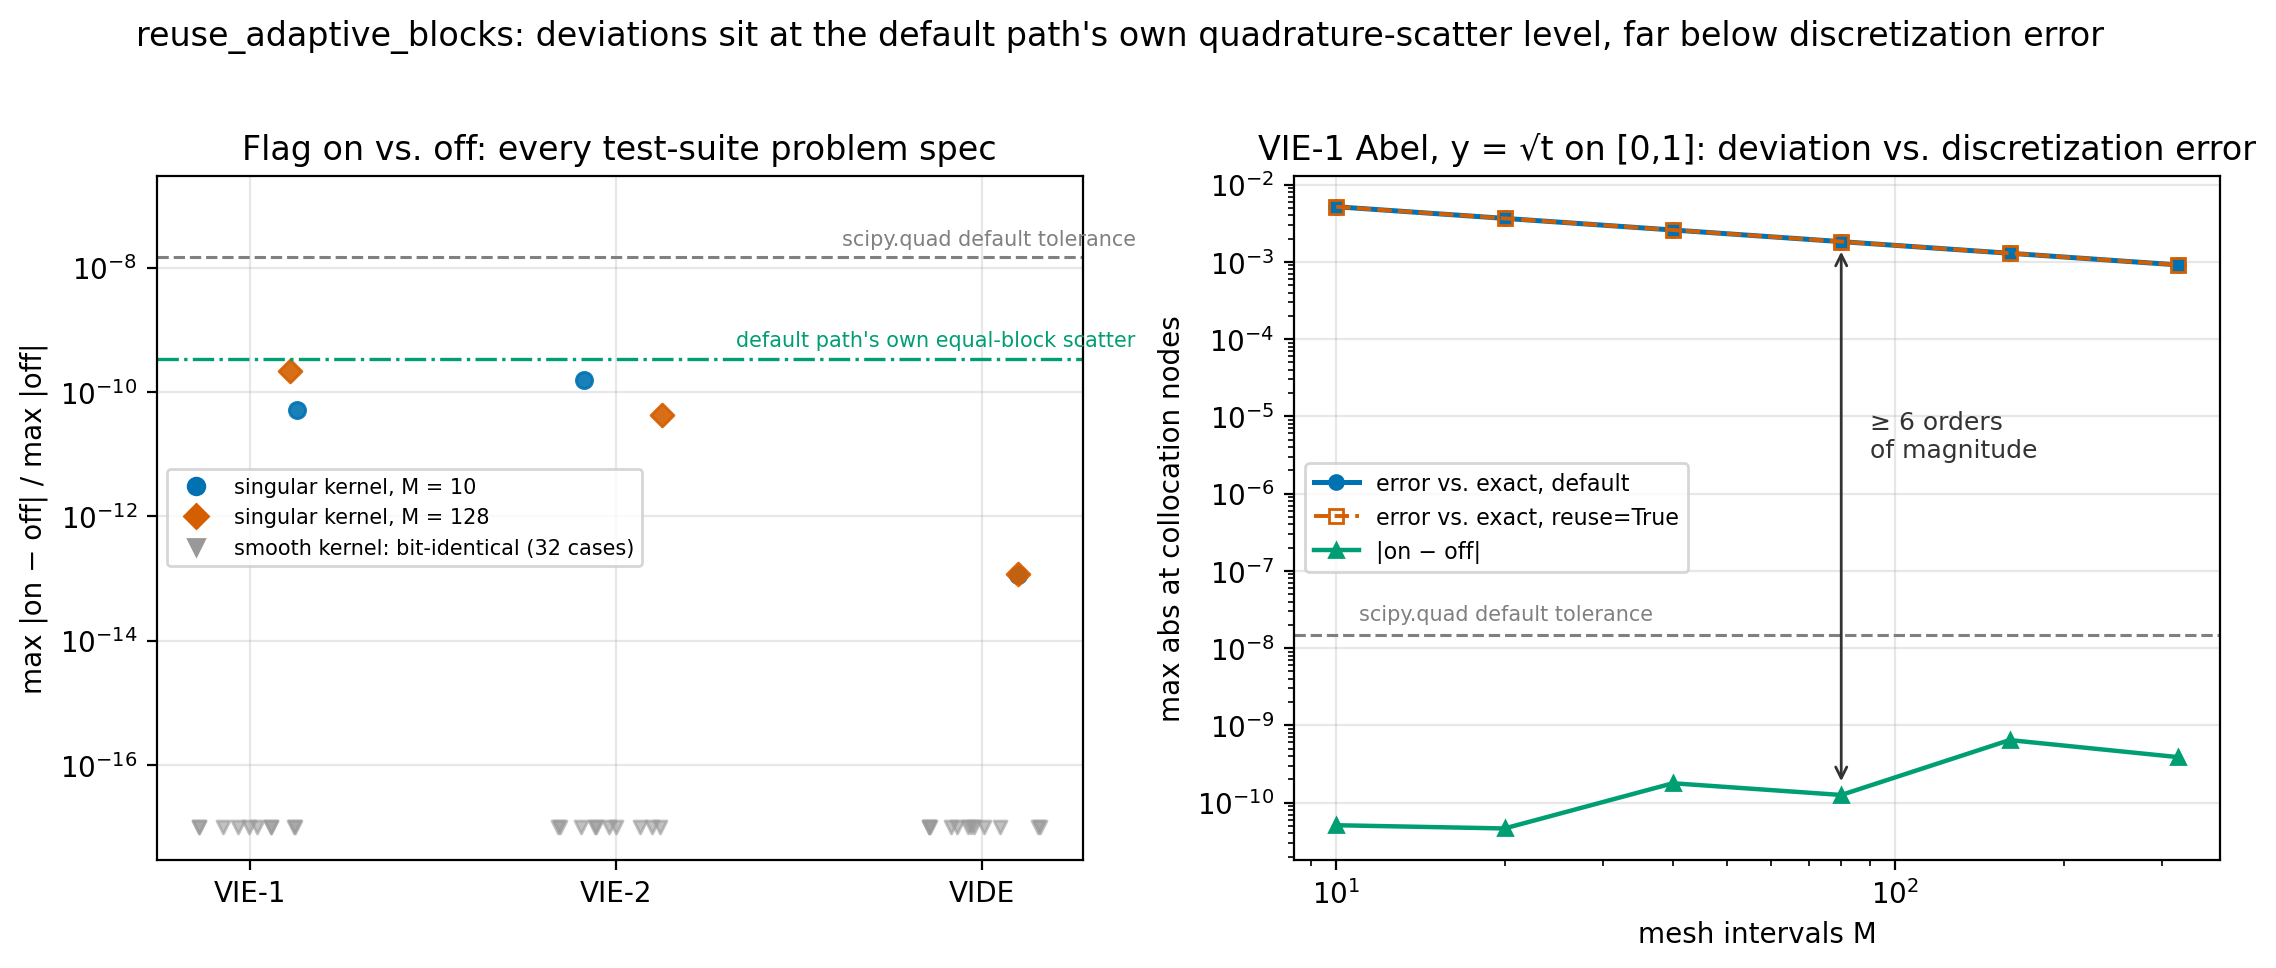
\includegraphics[width=\textwidth]{plot_reuse_differences.png}
\caption{Left: relative on/off deviation for every test-suite problem
spec (smooth kernels are bit-identical by construction). The green line
is the default path's own equal-block scatter; the deviations do not
exceed it. Right: on the $y=\sqrt{t}$ model problem, the deviation sits
six-plus orders of magnitude below the discretization error at every
mesh size.}
\label{fig:diff}
\end{figure}

\begin{table}[t]
\centering
\begin{tabular}{llcc}
\toprule
spec & solver & $M=10$ & $M=128$\\
\midrule
\texttt{VIE1\_SPEC\_ABEL} & VIE-1 & $5.1\times10^{-11}$ & $2.2\times10^{-10}$\\
\texttt{VIE2\_SPEC\_ABEL} & VIE-2 & $1.6\times10^{-10}$ & $4.3\times10^{-11}$\\
\texttt{VIDE\_SPEC\_ABEL} & VIDE  & $1.1\times10^{-13}$ & $1.2\times10^{-13}$\\
\midrule
\multicolumn{2}{l}{all 32 smooth-kernel cases} &
\multicolumn{2}{c}{bit-identical}\\
\bottomrule
\end{tabular}
\caption{Relative solution deviation, flag on vs.\ off, for every
problem spec of the test suite (scalar battery; uniform meshes on
$[0,1]$, $p=3$).}
\label{tab:battery}
\end{table}

Four observations, in decreasing order of force:
\begin{enumerate}
\item \textbf{The deviation does not exceed the error the default path
  already commits.} Anyone accepting the default output accepts
  quadrature errors of order $10^{-10}$ in the weights --- the default
  path's own equal-block scatter (Figure~\ref{fig:diff}, left).
  ``Different from the default'' here does not mean ``worse than the
  default'': both paths sit inside the same quadrature-error
  neighborhood of the exact tensor.
\item \textbf{The flagged path is, if anything, the more accurate one.}
  The reused blocks are computed at $10^{-12}$ tolerance, so each is
  closer to the exact integral than the $1.5\times10^{-8}$-tolerance
  per-row values it replaces. The on/off difference is dominated by the
  \emph{default} path's error. The flagged tensor is also exactly
  Toeplitz --- self-consistent in a way the default tensor is not.
\item \textbf{The deviation is invisible at the level of the
  computed solution.} On the $y=\sqrt t$ model problem the on/off
  difference sits $\ge 6$ orders below discretization error at every
  mesh size (Figure~\ref{fig:diff}, right); for well-scaled problems
  across the suite it never exceeds $2.2\times10^{-10}$ relative.
  Problems with growing resolvents amplify weight perturbations by
  their conditioning --- but they amplify the default path's quadrature
  error by exactly the same factor, so the flag does not change the
  achievable accuracy there either (e.g.\ a $d=2$ second-kind Abel
  system on $T=20$ with solution growth to $5\times10^{8}$: relative
  deviation $5\times10^{-8}$; the same system on $T=2$:
  $6\times10^{-10}$).
\item \textbf{The trade is scoped and reversible.} Default off; strict
  no-op guarantees on every path where it could surprise; one keyword
  to flip per call site.
\end{enumerate}

\noindent\textbf{When not to use it.} The flag is the wrong choice
whenever bitwise-stable outputs matter more than speed: regression
suites that pin archived outputs below $10^{-8}$, cross-run
reproducibility audits, or any comparison between flag-on and flag-off
outputs at tolerances tighter than the quadrature tolerance. That is
precisely why it is not the default.

\section{Verification}

All 369 repository tests pass (363 existing --- the default path is
untouched at rounding level --- plus 6 new tests covering: on/off
closeness for VIE-1, VIE-2, VIDE and a $d=2$ system; accuracy
unchanged against exact solutions; and the bit-identical no-op on
graded meshes and smooth kernels). The measurements in this note are
reproducible from the battery scripts accompanying the branch: every
test-suite problem spec run through both flag settings at two mesh
sizes, plus the equal-block scatter measurement on the default build.

\section{Outlook: getting both}

The principled way to keep the strict reproducibility criterion
\emph{and} this speed is to make the singular blocks deterministic:
replace QUADPACK on singularity-touching blocks by fixed-order
Gauss--Jacobi rules built for the weight $(b-s)^{-\alpha}$, with the
same two-order acceptance check used on the smooth path. Deterministic
rules are shift-stable to ulps, so those blocks would become reusable
under the same policy that already covers Gauss--Legendre --- no flag
needed, no tolerance-level deviations, and the Abel build would match
the smooth-kernel speed. This requires the singularity exponent
$\alpha$ (already supplied by users of \texttt{optimal\_graded\_mesh})
and is the natural follow-up.

\end{document}
